\section{Condition diagnostics and recorded failures}
\begin{figure}[htbp]
\centering
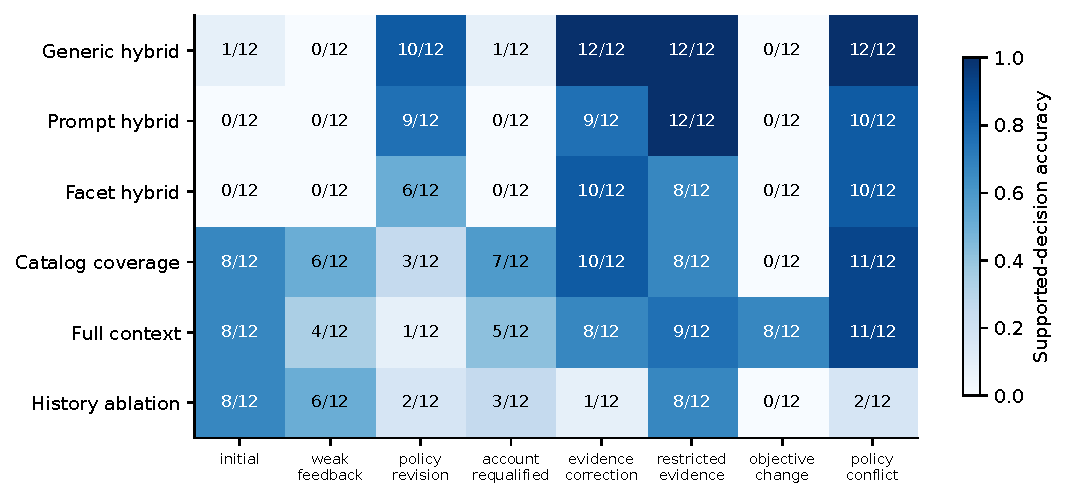
\includegraphics[width=\linewidth]{figures/primary/conditions.pdf}
\caption{Primary correct decisions out of 12 worlds per condition. Columns follow protocol order, not one uninterrupted timeline. Initial, weak-feedback, account-requalified and objective-change cases are positive; the other four require withholding. Each cell uses the same worlds, so the cells are not independent samples.}
\label{fig:conditions}
\end{figure}

\begin{table}[htbp]
\centering\small
\begin{tabular}{lrrrrr}
\toprule
Method & Decision & Positive & Neg. rec. & Tokens & Gen. sec. \\
\midrule
Prompt hybrid & 43.8\% & 27.1\% & 39.6\% & 1523 & 53.9 \\
Catalog coverage & 61.5\% & 62.5\% & 39.6\% & 1519 & 52.5 \\
\bottomrule
\end{tabular}

\caption{Exploratory 1,536-token comparison, with the same definitions and 96/48/48 denominators as Table~\ref{tab:primary}. These queries reuse the same 12 worlds, not a new independent sample.}
\end{table}

The error-localization script selects the first lexicographic case in each category, preserving all other examples and paired disagreements. The following inspections use those pointers. They are research-assistant readings of recorded traces, not blinded expert assessment or representative sampling.

\paragraph{Withholding despite complete support.}
For \texttt{q0b2e9ee8ab}, catalog-coverage attempt 167 binds the approved seller role/geography and observed account role/geography correctly. Its qualification alternative has no additional requirements. The output nevertheless requests partner status, channel fit, offering pain and procurement stage. Full-context attempt 211 instead selects the valid qualification alternative. This records failure to scope missing information to the requested alternative, despite the clarified common instructions.

\paragraph{Inapplicable recommendation with correct source bindings.}
For \texttt{q0d8088c402}, catalog-coverage attempt 516 recommends template P1. The supplied approved seller geography is UK, while the account geography is EU; the template also costs three units against a two-unit allowance. Its prerequisite table points to the actual supplied records. Correctly naming records therefore does not establish that their values satisfy equality or resource constraints. The scorer records an inapplicable template and prevents mock execution.

\paragraph{Proposal mistaken for approved policy.}
For \texttt{q1c366e6ee1}, catalog-coverage attempt 226 binds the approved-geography slot to S9, an unapproved CA proposal, instead of S2, the approved UK policy matching the account. The raw output and original bindings remain intact. The scorer rejects misbound, incomplete and irrelevant support; it does not silently substitute S2. This error illustrates why authority metadata must be checked in the decision, even when it is preserved in memory.
